
\documentclass[11pt]{exam} % https://www.ctan.org/pkg/exam?lang=en

\usepackage[lmargin=1.in,rmargin=1.in,tmargin=1.in,bmargin=1in]{geometry}
\usepackage{setspace}
\usepackage[pdftex]{graphicx}
\usepackage{titling}
\usepackage[
	pdfauthor={Brian Weinstein},
	pdftitle={Homework 1},
	bookmarks=true,
	colorlinks=true,
	linkcolor=blue,
	urlcolor=blue,
	citecolor=blue,
	pdftex,
	linktocpage=true
	]{hyperref}
\usepackage[textsize=tiny]{todonotes}
\usepackage{float}
\setlength\parindent{0pt} % or 1em
\usepackage{lipsum}
\usepackage{amsmath}
\usepackage{caption}


\qformat{\textbf{Problem \thequestion: \thequestiontitle}\quad \hfill}


\pagestyle{headandfoot}
\runningheadrule
\firstpageheader{}{}{}
\runningheader{\theauthor}{\thetitle}{\thedate}
\firstpagefooter{}{\thepage}{}
\runningfooter{}{\thepage}{}


\usepackage{xcolor}
\usepackage{adjustbox}
\usepackage{verbatim}
\definecolor{shadecolor}{rgb}{.9, .9, .9}

\newenvironment{code}%
   {\par\noindent\adjustbox{margin=1ex,bgcolor=shadecolor,margin=0ex \medskipamount}\bgroup\minipage\linewidth\verbatim}%
   {\endverbatim\endminipage\egroup}

\newenvironment{codeSmall}%
   {\par\noindent\adjustbox{margin=1ex,bgcolor=shadecolor,margin=0ex \medskipamount}\bgroup\minipage\linewidth\verbatim\footnotesize}%
   {\endverbatim\endminipage\egroup}

\newcommand{\ramsey}{\href{http://www.statisticalsleuth.com/}{Ramsey }}



\begin{document}


\title{STAT W4201 001, Homework 7}
\author{Brian Weinstein (bmw2148)}
\date{Mar 28, 2016}
\maketitle

Code is attached here and also posted at \href{https://github.com/BrianWeinstein/advanced-data-analysis}{https://github.com/BrianWeinstein/advanced-data-analysis}. Where relevant, code snippets and output are are included in-line.

\begin{questions}


\titledquestion{\ramsey 10.21}

Let

$$
\mathbf{Y} = 
  \begin{bmatrix}
    Y_1 \\
    Y_2 \\
    \vdots \\
    Y_n
  \end{bmatrix}
, \quad
\mathbf{X}=
  \begin{bmatrix}
    1 & X_{11} & X_{12} & \cdots & X_{1p} \\
    1 & X_{21} & X_{22} & \cdots & X_{2p} \\
    \vdots & \vdots & \vdots &  & \vdots \\
    1 & X_{n1} & X_{n2} & \cdots & X_{np} \\
  \end{bmatrix}
, \quad \text{and \ }
\mathbf{b} = 
  \begin{bmatrix}
    \beta_0 \\
    \beta_1 \\
    \vdots \\
    \beta_p
  \end{bmatrix} .
$$

By deconstructing $(\mathbf{X}^T \mathbf{X}) \mathbf{b} = \mathbf{X}^T \mathbf{Y}$ we find the set of normal equations:
\begin{gather*}
(\mathbf{X}^T \mathbf{X}) \mathbf{b} = \mathbf{X}^T \mathbf{Y} \\ 
\Rightarrow \left(
  \begin{bmatrix}
  	1 & 1 & \cdots & 1 \\
  	X_{11} & X_{21} & \cdots & X_{n1} \\
  	X_{12} & X_{22} & \cdots & X_{n2} \\
    \vdots & \vdots &  & \vdots \\
  	X_{1p} & X_{2p} & \cdots & X_{np} \\
  \end{bmatrix}
  \begin{bmatrix}
    1 & X_{11} & X_{12} & \cdots & X_{1p} \\
    1 & X_{21} & X_{22} & \cdots & X_{2p} \\
    \vdots & \vdots & \vdots &  & \vdots \\
    1 & X_{n1} & X_{n2} & \cdots & X_{np} \\
  \end{bmatrix}
\right)
\begin{bmatrix}
    \beta_0 \\
    \beta_1 \\
    \vdots \\
    \beta_p
  \end{bmatrix}
=
  \begin{bmatrix}
  	1 & 1 & \cdots & 1 \\
  	X_{11} & X_{21} & \cdots & X_{n1} \\
  	X_{12} & X_{22} & \cdots & X_{n2} \\
    \vdots & \vdots &  & \vdots \\
  	X_{1p} & X_{2p} & \cdots & X_{np} \\
  \end{bmatrix}
  \begin{bmatrix}
    Y_1 \\
    Y_2 \\
    \vdots \\
    Y_n
  \end{bmatrix}
\\
\Rightarrow \begin{bmatrix}
  	n & \sum X_{i1} & \sum X_{i2} & \cdots & \sum X_{ip} \\
  	\sum X_{i1} & \sum X_{i1}^2 & \sum X_{i1} X_{i2 } & \cdots & \sum X_{i1} X_{ip} \\
  	\sum X_{i2} & \sum X_{i2} X_{i1} & \sum X_{i2}^2 & \cdots & \sum X_{i2} X_{ip} \\
  	\vdots & \vdots & \vdots &  & \vdots \\
  	\sum X_{ip} & \sum X_{ip} X_{i1} & \sum X_{ip} X_{i2} & \cdots & \sum X_{ip}^2 \\
  \end{bmatrix}
  \begin{bmatrix}
    \beta_0 \\
    \beta_1 \\
    \vdots \\
    \beta_p
  \end{bmatrix}
=
  \begin{bmatrix}
    \sum Y_{i} \\
    \sum X_{i1} Y_i \\
    \sum X_{i2} Y_i \\
    \vdots \\
    \sum X_{ip} Y_i \\
  \end{bmatrix}
\\
\Rightarrow \begin{bmatrix}
  	\beta_0 n + \beta_1 \sum X_{i1} + \beta_2 \sum X_{i2} + \cdots + \beta_p \sum X_{ip} \\
  	\beta_0 \sum X_{i1} + \beta_1 \sum X_{i1}^2 + \beta_2 \sum X_{i1} X_{i2 } + \cdots + \beta_p \sum X_{i1} X_{ip} \\
  	\beta_0 \sum X_{i2} + \beta_1 \sum X_{i2} X_{i1} + \beta_2 \sum X_{i2}^2 + \cdots + \beta_p \sum X_{i2} X_{ip} \\
  	\vdots \\
  	\beta_0 \sum X_{ip} + \beta_1 \sum X_{ip} X_{i1} + \beta_2 \sum X_{ip} X_{i2} + \cdots + \beta_p \sum X_{ip}^2 \\
  \end{bmatrix}
=
  \begin{bmatrix}
    \sum Y_{i} \\
    \sum X_{i1} Y_i \\
    \sum X_{i2} Y_i \\
    \vdots \\
    \sum X_{ip} Y_i \\
  \end{bmatrix} ,
\end{gather*}
where each $\sum$ indicates summation over all cases ($i = 1, 2, \ldots, n$).

As long as $\mathbf{X}^T \mathbf{X}$ is invertible, the least squares solution is $\mathbf{b} = (\mathbf{X}^T \mathbf{X})^{-1} \mathbf{X}^T \mathbf{Y}$. By the invertible matrix theorem, $\mathbf{X}^T \mathbf{X}$ is invertible whenever the columns of $\mathbf{X}$ are linearly independent.

\titledquestion{\ramsey 10.22}
\todo{Problem 2: 10.22}


\titledquestion{\ramsey 10.26}
\textit{Does the effect of UVB exposure on the distribution of percentage inhibition differ at the surface and in the deep? How much difference is there? Analyze the data, and write a summary of statistical findings and a section of details documenting those findings.}

A sample of the dataset is shown below, and a coded scatterplot of the \texttt{Inhibit} vs \texttt{UVB} is shown in Figure \ref{fig:3_eda}.

\begin{codeSmall}
   Inhibit  UVB Surface
1      0.0 0.00       0
2      1.0 0.00       0
3      6.0 0.01       0
4      7.0 0.01       1
...
14    21.0 0.04       1
15    25.0 0.02       0
16    39.0 0.03       0
17    59.0 0.03       0
\end{codeSmall}

\begin{figure}[!h]
	\centering
	\captionsetup{width=0.8\textwidth}
	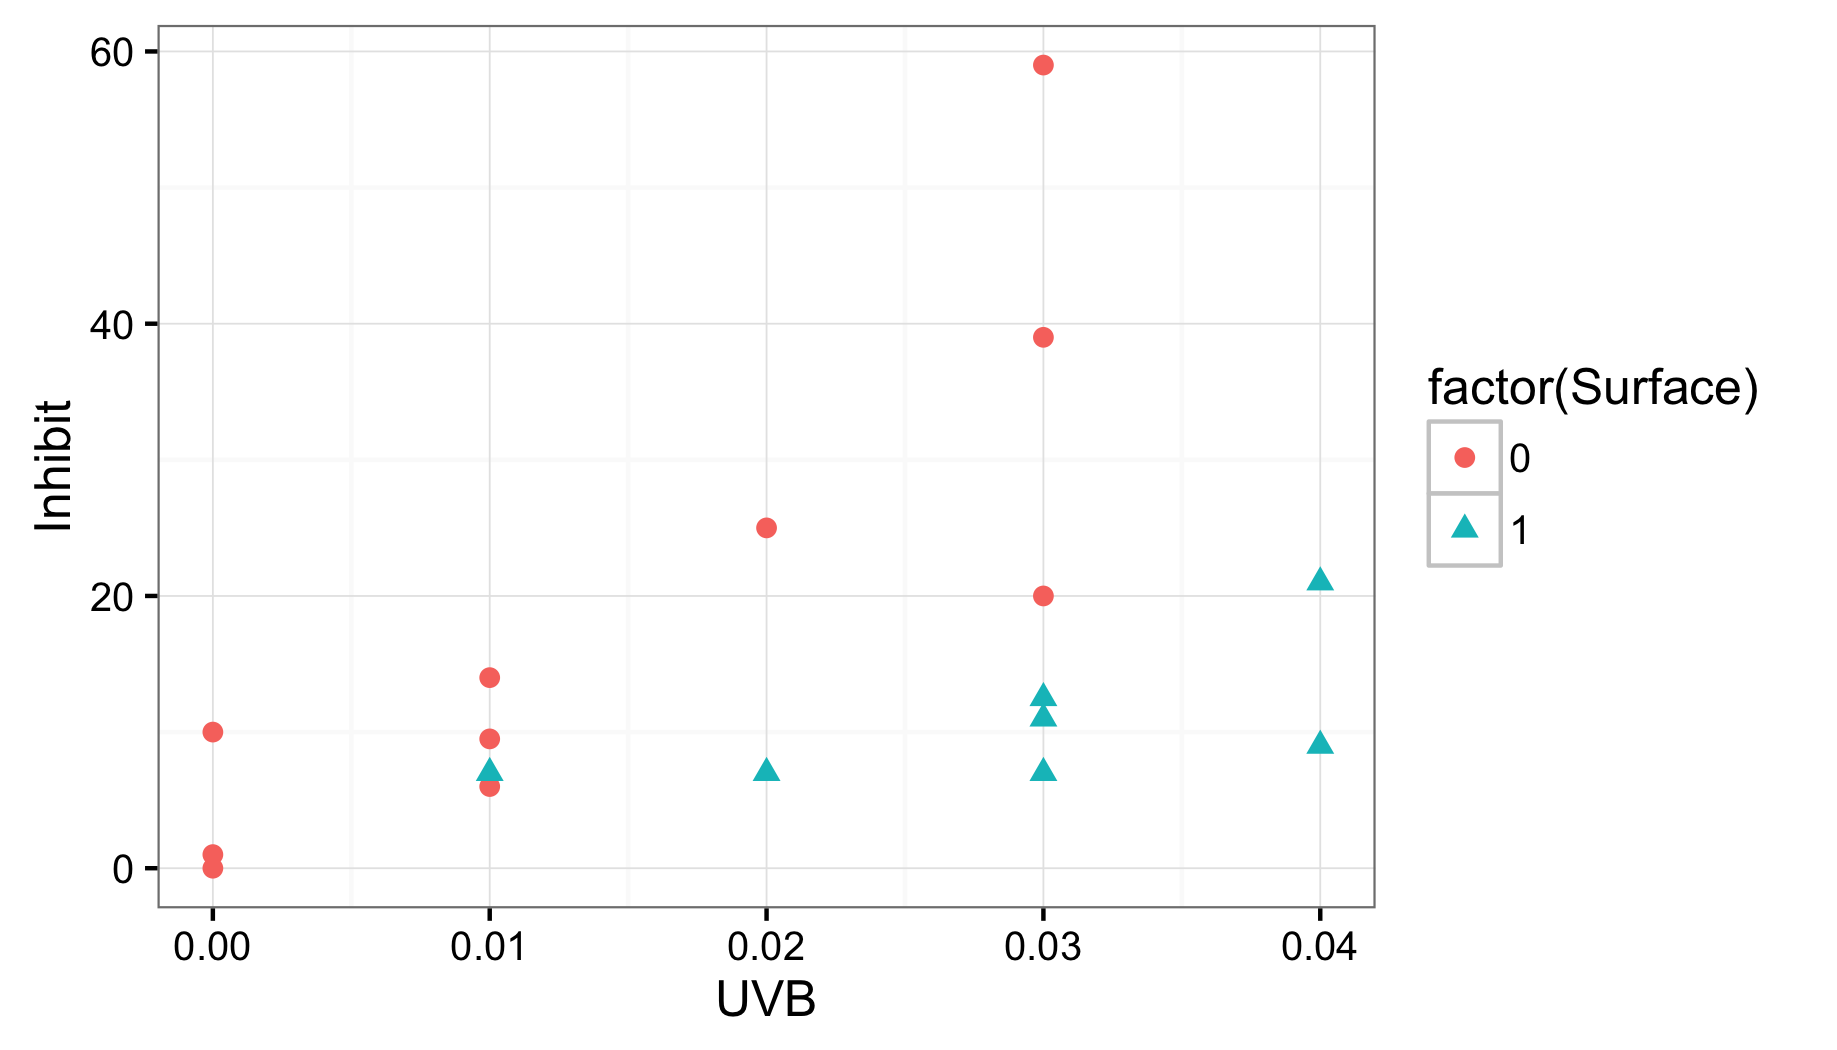
\includegraphics[width=4.25in]{3_eda.png}
	\caption{Coded scatterplot of \texttt{Inhibit} vs \texttt{UVB}. \texttt{Surface} = 1 indicates a measurement close to the surface, and \texttt{Surface} = 0 in deep water.}
	\label{fig:3_eda}
\end{figure}

First, we fit a linear model on the full dataset, including an interaction term between \texttt{UVB} and \texttt{Surface}.

\begin{codeSmall}
> lmFull <- lm(Inhibit ~ Surface*UVB, data=ozoneData)
> summary(lmFull)$coefficients
               Estimate Std. Error    t value     Pr(>|t|)
(Intercept)    1.180556   4.292122  0.2750517 0.7875994449
Surface        1.277778  11.065902  0.1154698 0.9098372976
UVB         1226.388889 232.772995  5.2686047 0.0001518894
Surface:UVB -939.930556 409.839150 -2.2934133 0.0391340538
\end{codeSmall}$

In this model, the p-value on the intercept term indicates that the data provides no evidence to suggest that the intercept is non-zero. Based on the dataset, we also know the intercept should be nearly 0 for both the surface-level and deep water measurements. We fit a second model, forcing the intercept term to 0.

\begin{codeSmall}
> lmZeroInt <- lm(Inhibit ~ 0 + Surface*UVB, data=ozoneData)
> summary(lmZeroInt)$coefficients
               Estimate Std. Error    t value      Pr(>|t|)
Surface        2.458333   9.857139  0.2493962 0.80667620946
UVB         1275.000000 146.400333  8.7089966 0.00000050281
Surface:UVB -988.541667 357.358785 -2.7662442 0.01515365491
\end{codeSmall}$

Although the model with 0-intercept has a slightly higher RMSE, the difference is negligible (8.537, vs 8.833 in the full model), and the significance of the coefficients is unchanged.

Based on the full model, the data provides moderate evidence that the effect of UVB exposure on the distribution of percentage inhibition differs at the surface and in the deep (two sided p-value of $0.03913$, from a test that the \texttt{Surface:UVB} coefficient estimate is 0; estimated value $-939.9$, 95\% CI from -1825 to -54.53). In deep water, for each 0.01 unit increase in UVB exposure, the percent inhibition increases by 12.26 percentage points. Near the surface, however, for each 0.01 unit increase in UVB exposure, the percent inhibition increases by only 2.861 percentage points.

The regression equations for this ``separate lines'' model are shown below
\begin{itemize}
\item Near the surface ($\texttt{Surface} = 1$): $\texttt{Inhibit} = 3.084 + 286.1 \times \texttt{UVB}$,
\item and in deep water ($\texttt{Surface} = 0$): $\texttt{Inhibit} = 1.806 + 1226 \times \texttt{UVB}$.
\end{itemize}

\titledquestion{\ramsey 11.8}

\begin{parts}

\part \textit{Why does a case with large leverage have the potential to be influential? Why is it not necessarily influential?}

An observation with large leverage $h_i$ has a residual with low variability
$$\text{SD}(\text{Residual}_i) = \sigma \sqrt{1-h_i}.$$ A high-leverage observation's explanatory variable values are abnormally high or low, as compared to the other observations in the dataset. As such, the high-leverage observation determines the value of the regression in the surrounding region.

This, however, does not mean that all high-leverage observations are influential. If the observation happens to fall close to the regression surface that is fit only to the other observations (i.e., excluding the high-leverage observation), then the high-leverage observation has little impact on the overall regression surface.

\part \textit{Draw a hypothetical scatterplot of Y versus a single X, where one observation has a high leverage but is not influential.}

A scatterplot with a high-leverage, low-influence observation is shown in Figure \ref{fig:4b}.

\begin{figure}[!h]
	\centering
	\captionsetup{width=0.8\textwidth}
	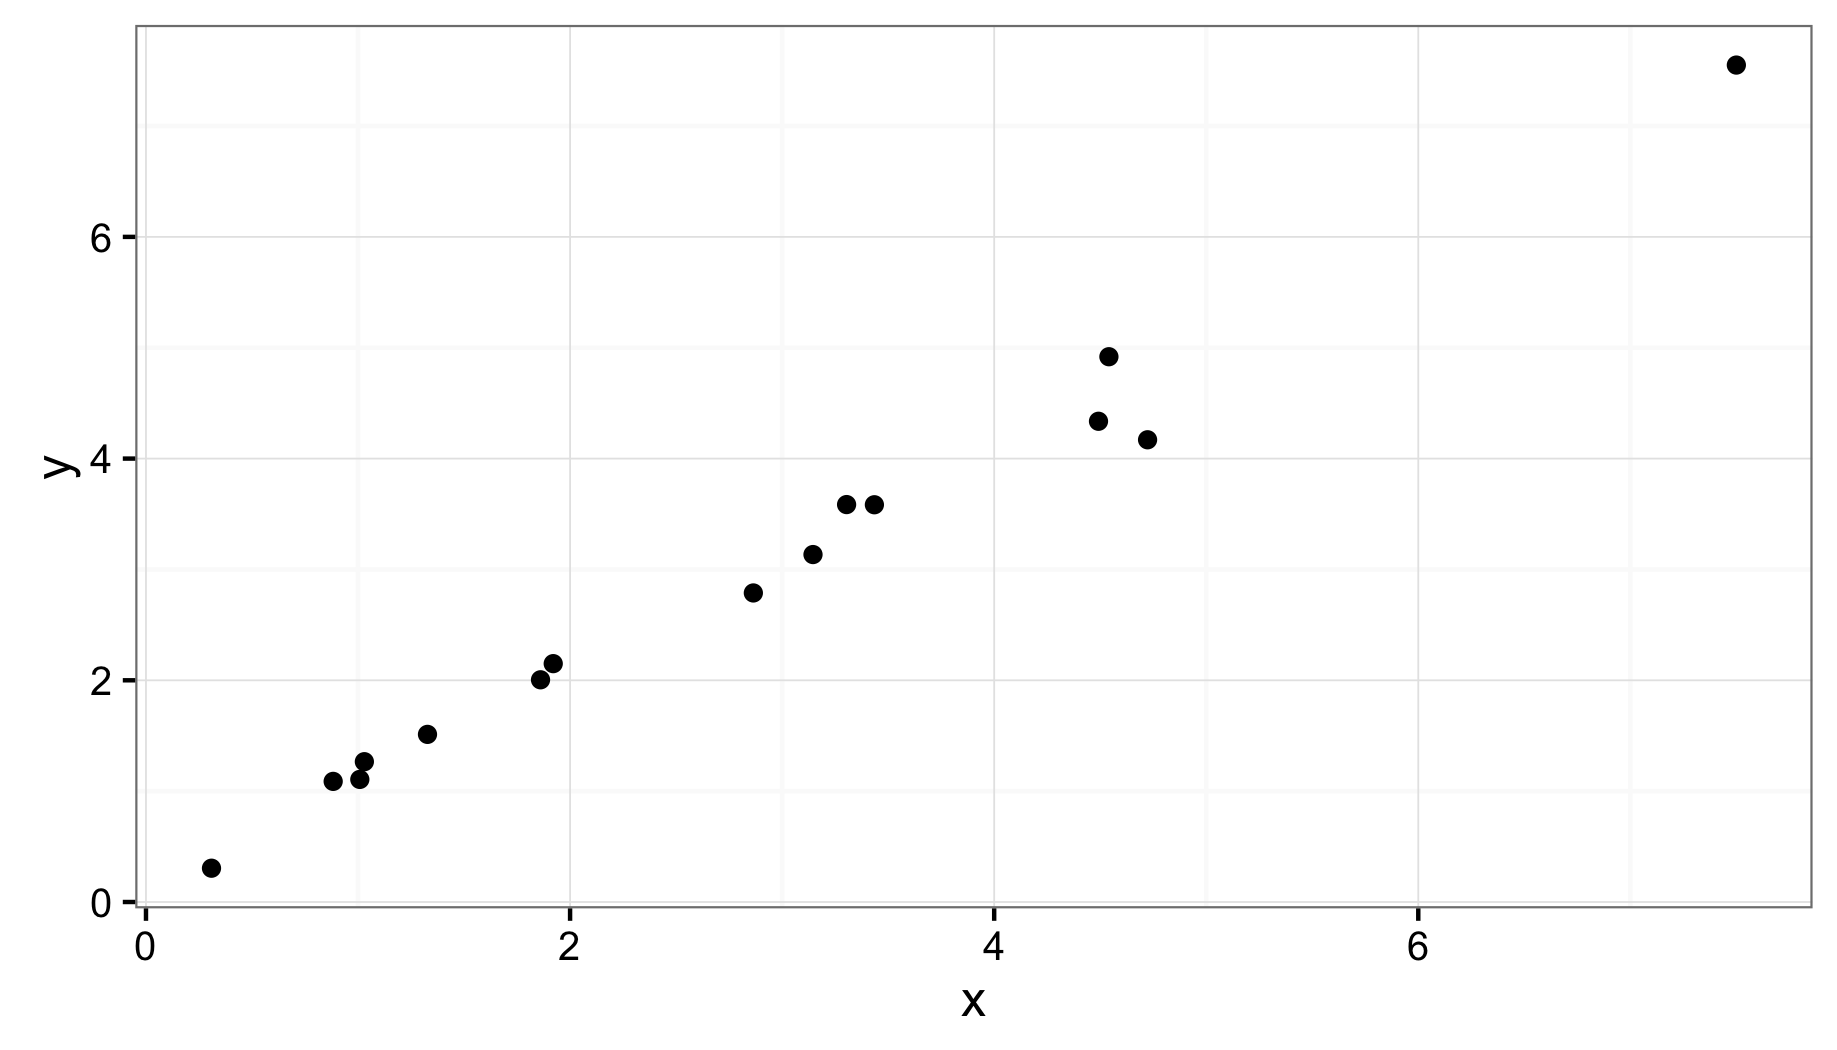
\includegraphics[width=4in]{4b.png}
	\caption{A scatterplot with a high-leverage, low-influence observation.}
	\label{fig:4b}
\end{figure}

\part \textit{Draw a hypothetical scatterplot of Y versus a single X, where one observation has a high leverage and is influential.}

A scatterplot with a high-leverage, high-influence observation is shown in Figure \ref{fig:4c}.

\begin{figure}[!h]
	\centering
	\captionsetup{width=0.8\textwidth}
	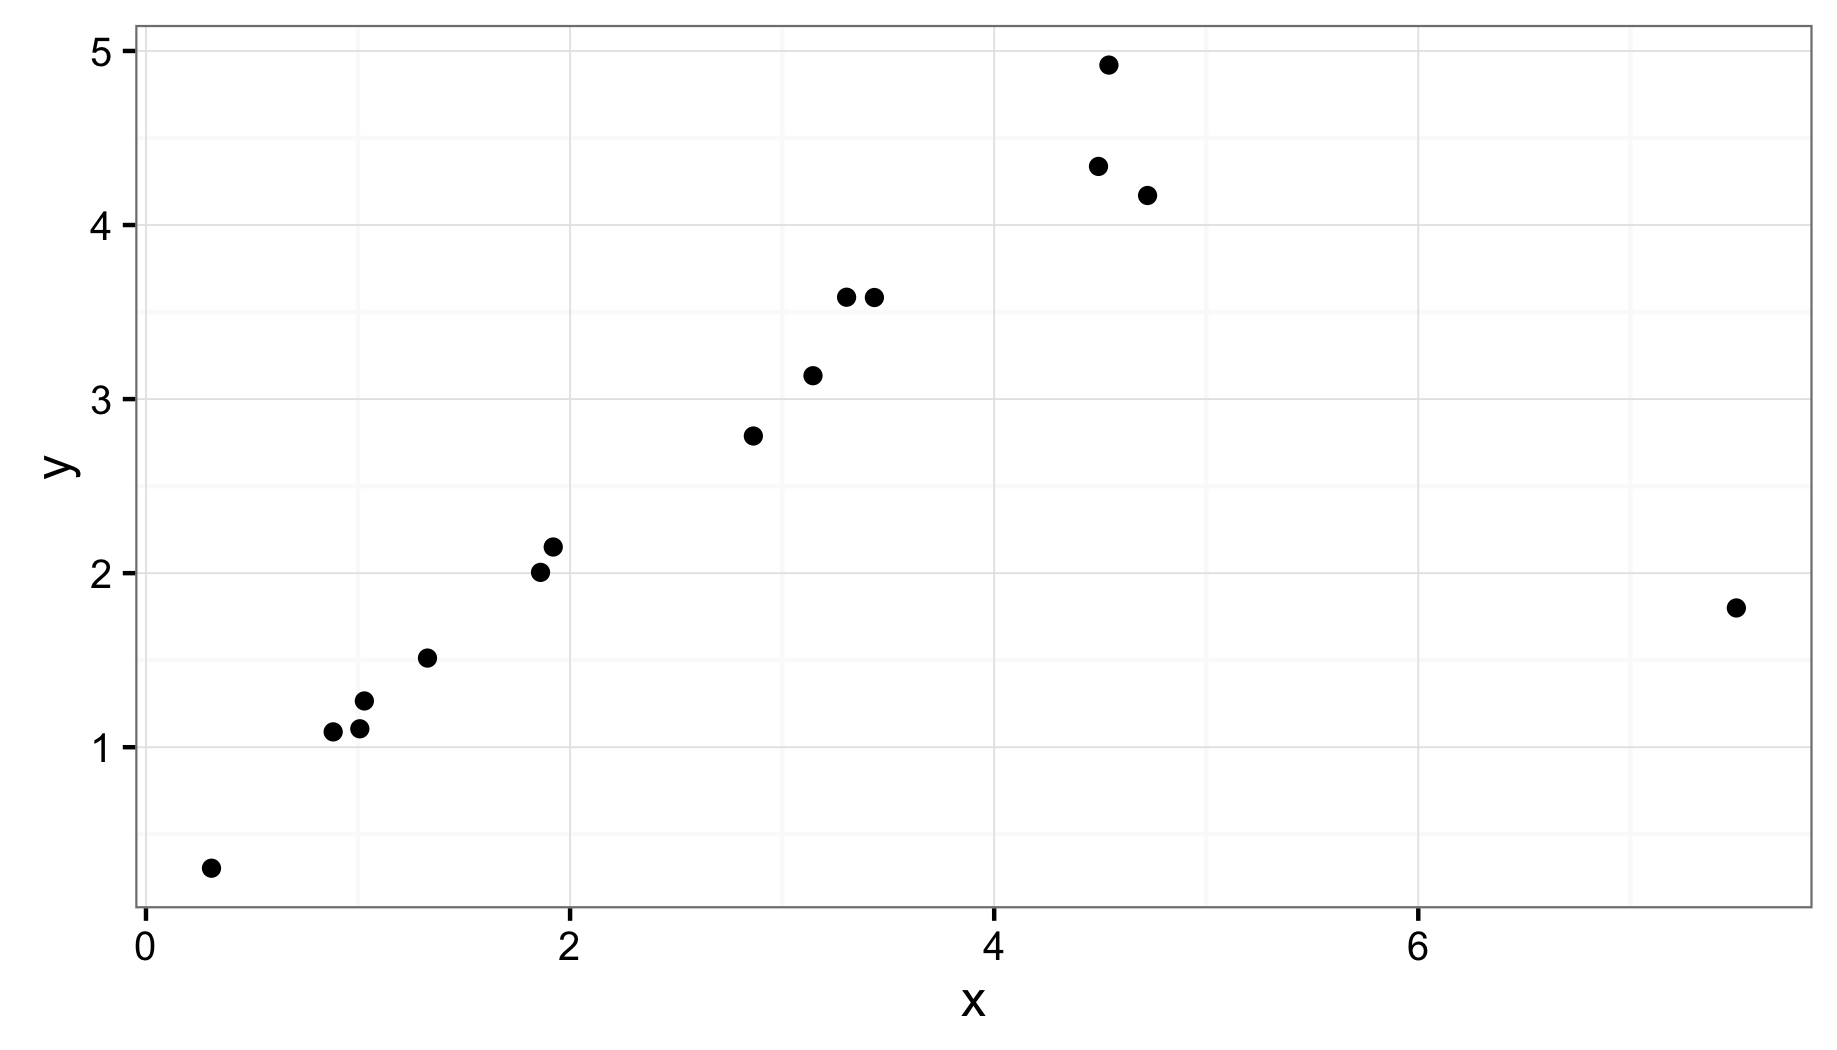
\includegraphics[width=4in]{4c.png}
	\caption{A scatterplot with a high-leverage, high-influence observation.}
	\label{fig:4c}
\end{figure}

\end{parts}

\titledquestion{\ramsey 11.16}

\textit{Calculate the leverage, the studentized residual, and Cook’s Distance for the 32nd case. Use the model with gastric activity, a sex indicator variable, and the interaction of these two.}

The regression of \texttt{Metabol} on \texttt{Gastric}, \texttt{Sex}, and their interaction is shown below, and a coded scatterplot is shown in Figure \ref{fig:5}.

\begin{codeSmall}
> lmFpm <- lm(formula = Metabol ~ Gastric*Sex, data = fpmData)
> summary(lmFpm)$coefficients
                  Estimate Std. Error    t value   Pr(>|t|)
(Intercept)     -0.1972691  0.8022017 -0.2459096 0.80754593
Gastric          0.8369478  0.4838925  1.7296153 0.09471027
SexMale         -0.9884969  1.0723910 -0.9217691 0.36452374
Gastric:SexMale  1.5069236  0.5591376  2.6950856 0.01176490
\end{codeSmall}$

\begin{figure}[!h]
	\centering
	\captionsetup{width=0.8\textwidth}
	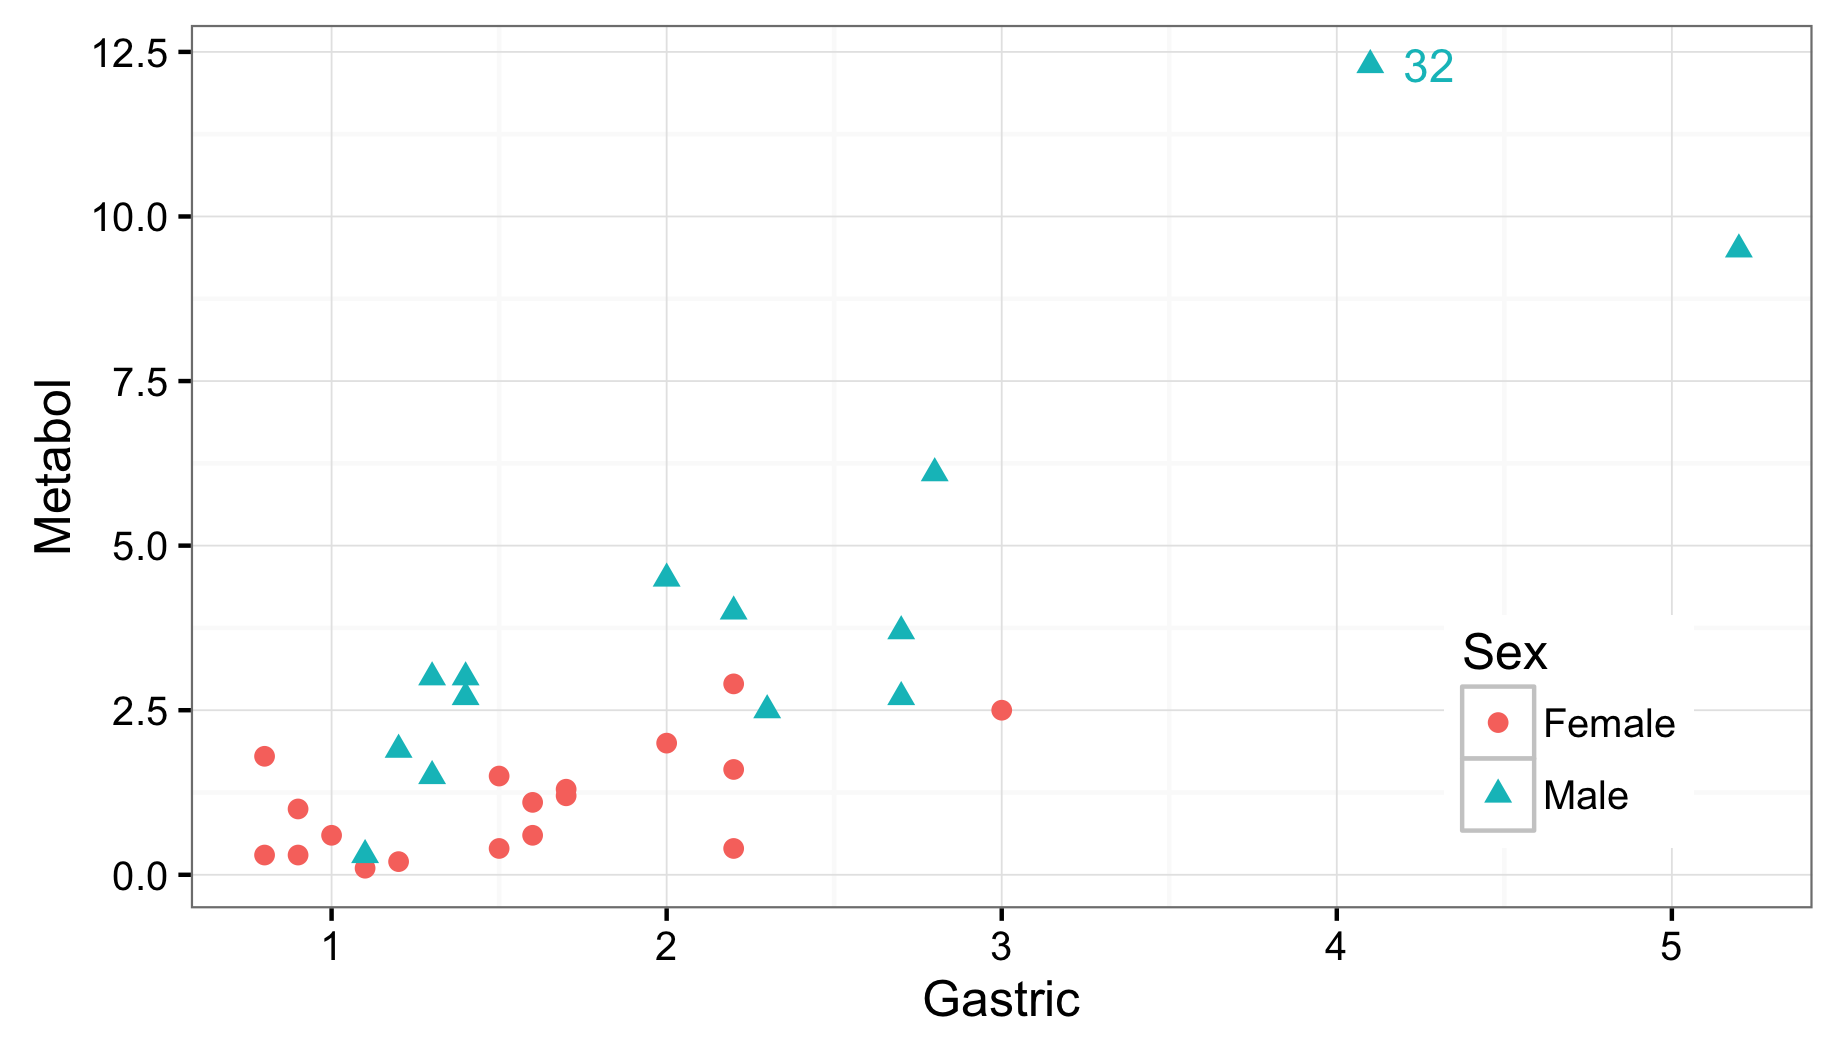
\includegraphics[width=4.25in]{5.png}
	\caption{Coded scatterplot of \texttt{Metabol} vs \texttt{Gastric}.}
	\label{fig:5}
\end{figure}

The leverage, studentized residual, and Cook's Distance for case 32 are shown below.
\begin{codeSmall}
> # calculate leverage for case 32
> hatvalues(lmFpm)[32]
       32 
0.2528749 
> # calculate the studentized residual for case 32
> studres(lmFpm)[32]
      32 
5.120516 
> # calculate Cook's Distance for case 32
> cooks.distance(lmFpm)[32]
      32 
1.167255 
\end{codeSmall}


\titledquestion{\ramsey 11.20}



\end{questions}

\listoftodos

\end{document}